\documentclass[10pt,a4paper,parskip=half]{scrartcl}
\usepackage[utf8]{inputenc}
\usepackage{amsmath}
\usepackage{amsfonts}
\usepackage{amssymb}
\usepackage{mathpazo}
\usepackage{tikz}
\usetikzlibrary{patterns}
\usepackage{stmaryrd} % Für den Widerspruchsblitz :D
\usepackage[left=1cm, right=1cm,
top=1cm, bottom=1cm]{geometry}
\usepackage{fullpage}
\usepackage[german]{babel}
\usepackage{enumerate}
\setlength{\unitlength}{1cm}
\newcommand{\N}{\mathbb{N}}
\newcommand{\A}{\mathcal{A}}
\newcommand{\R}{\mathbb{R}}
\parindent 0mm
\author{Tom}
\title{Analysis 2 - Hausaufgabe 12}

% new commands for vectors
\newcommand{\vectwo}[2]{\begin{pmatrix}#1\\#2\\\end {pmatrix}}
\newcommand{\vecthree}[3]{\begin{pmatrix}#1\\#2\\#3\\\end {pmatrix}}

\usepackage{listings}
\usepackage{courier}
 \lstset{
         basicstyle=\footnotesize\ttfamily, % Standardschrift
         %numbers=left,               % Ort der Zeilennummern
         numberstyle=\tiny,          % Stil der Zeilennummern
         %stepnumber=2,               % Abstand zwischen den Zeilennummern
         numbersep=5pt,              % Abstand der Nummern zum Text
         tabsize=2,                  % Groesse von Tabs
         extendedchars=true,         %
         breaklines=true,            % Zeilen werden Umgebrochen
         keywordstyle=\color{red},
      frame=b,         
 %        keywordstyle=[1]\textbf,    % Stil der Keywords
 %        keywordstyle=[2]\textbf,    %
 %        keywordstyle=[3]\textbf,    %
 %        keywordstyle=[4]\textbf,   \sqrt{\sqrt{}} %
         stringstyle=\color{white}\ttfamily, % Farbe der String
         showspaces=false,            % Leerzeichen anzeigen ?
         showtabs=false,              % Tabs anzeigen ?
         xleftmargin=17pt,
         framexleftmargin=17pt,
         framexrightmargin=5pt,
         framexbottommargin=4pt,
         %backgroundcolor=\color{lightgray},
         showstringspaces=false      % Leerzeichen in Strings anzeigen ?        
 }
 \usepackage{caption}
\DeclareCaptionFont{white}{\color{white}}
\DeclareCaptionFormat{listing}{\colorbox[cmyk]{0.43, 0.35, 0.35,0.01}{\parbox{\textwidth}{\hspace{15pt}#1#2#3}}}
\captionsetup[lstlisting]{format=listing,labelfont=white,textfont=white, singlelinecheck=false, margin=0pt, font={bf,footnotesize}}

\usepackage{color}
\usepackage{enumerate}



\begin{document}
\begin{center}
\textsc{\Large{Analysis 2 - Hausaufgabe 12}} \\
\end{center}
\begin{tabbing}
Tom Nick \hspace{1.4cm}\= 342225\\
Tom Lehmann\> 340621\\
Maximilian Bachl\> 341455
\end{tabbing}
\subsection*{1. Aufgabe}
\begin{enumerate}[(a)]
   \item \ \\
   \begin{minipage}{0.50\columnwidth}
   Ein Vollzylinder mit der Höhe 3 und dem Radius 2.
   \begin{lstlisting}[caption= Mathematica Code für die Menge Z]
   RegionPlot3D[x^2 + y^2 <= 4, {x, -2, 2}, {y, -2, 2}, {z, 0, 3}, 
   AxesLabel -> {x, y, z}]
   \end{lstlisting}
   \end{minipage}
   \begin{minipage}{0.50\columnwidth}
   \begin{center}
   \includegraphics[scale=0.7]{1aZ.pdf} 
   \end{center}
   \end{minipage}
   \item   \ \\
   \begin{minipage}{0.50\columnwidth}
   Ein VollKegel mit der Höhe 1.
   \begin{lstlisting}[caption= Mathematica Code für die Menge K]
   RegionPlot3D[
    Sqrt[x^2 + y^2] <= 8 - 2 z, {x, -8, 8}, 
    {y, -8, 8}, {z, 3, 4}, 
    AxesLabel -> {x, y, z}]
   \end{lstlisting}
   \end{minipage}
   \begin{minipage}{0.50\columnwidth}
   \begin{center}
   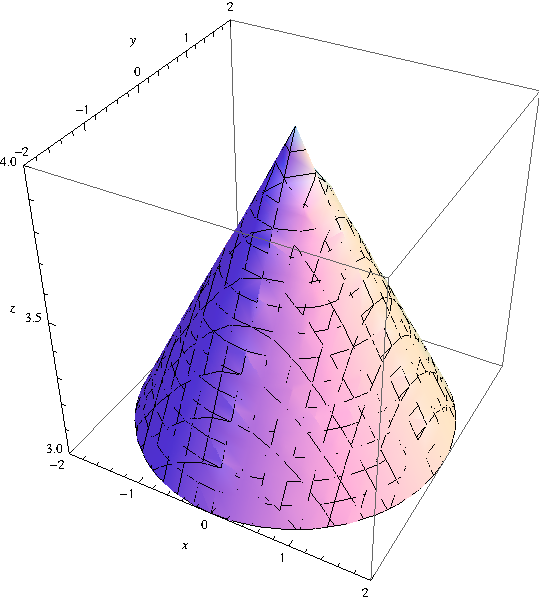
\includegraphics[scale=0.7]{1aK.pdf} 
   \end{center}
   \end{minipage}
\end{enumerate}

\end{document}

